\documentclass[tikz,border=8pt]{standalone}
\usetikzlibrary{arrows.meta,positioning}
\begin{document}
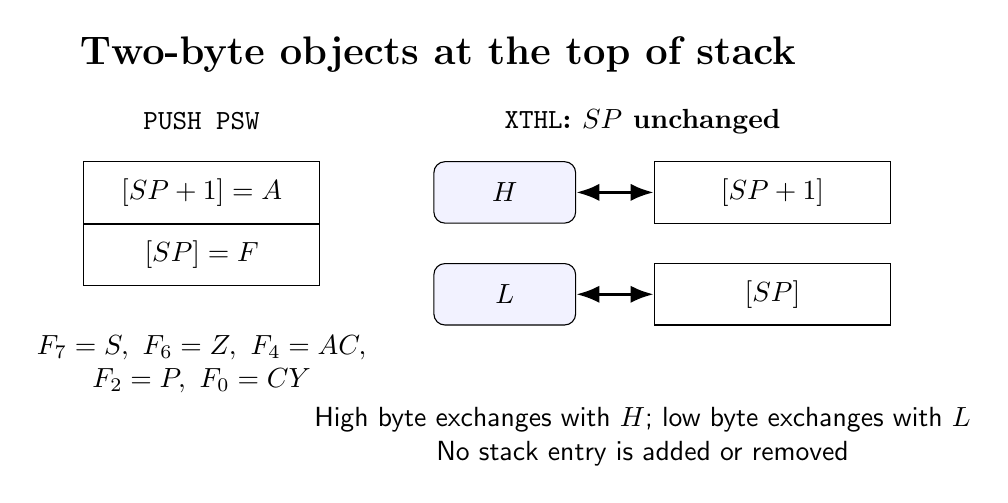
\begin{tikzpicture}[font=\sffamily,>=Latex,byte/.style={draw,minimum width=3.0cm,minimum height=.78cm,align=center},reg/.style={draw,rounded corners,minimum width=1.8cm,minimum height=.78cm,fill=blue!5}]
\node[font=\Large\bfseries] at (5.4,5.1) {Two-byte objects at the top of stack};
\node[font=\bfseries] at (2.4,4.25) {\texttt{PUSH PSW}};
\node[byte] (fa) at (2.4,3.35) {$[SP+1]=A$};
\node[byte,below=0pt of fa] (ff) {$[SP]=F$};
\node[below=5mm of ff,align=center] {$F_7=S,\ F_6=Z,\ F_4=AC,$\\$F_2=P,\ F_0=CY$};
\node[font=\bfseries] at (8.0,4.25) {\texttt{XTHL}: $SP$ unchanged};
\node[reg] (h) at (6.25,3.35) {$H$};
\node[reg,below=5mm of h] (l) {$L$};
\node[byte] (mh) at (9.65,3.35) {$[SP+1]$};
\node[byte,below=5mm of mh] (ml) {$[SP]$};
\draw[very thick,<->] (h)--(mh);
\draw[very thick,<->] (l)--(ml);
\node[align=center] at (8.0,.25) {High byte exchanges with $H$; low byte exchanges with $L$\\No stack entry is added or removed};
\end{tikzpicture}
\end{document}
